\let\RaggedRight\raggedright
\let\raggedright\relax
\documentclass[utf8,9pt,mathserif,usepdftitle=false]{beamer}
\usepackage[russian]{babel}

\newcommand{\dd}{\mathrm{d}}
\renewcommand{\Re}{\operatorname{Re}}
\renewcommand{\Im}{\operatorname{Im}}
\renewcommand{\exp}{\operatorname{e}}
\renewcommand{\imath}{\mathrm{i}}

% \input{present.daf}

% \setbeameroption{show notes on second screen}
\setbeameroption{hide notes}
\mode<presentation>
{
  \usetheme{default}
  %\usecolortheme{default} % dove, beaver
  \usecolortheme{whale}
  %\usefonttheme{serif}
}

\hypersetup{%
  pdfinfo={%
    Title={Lyapunov conference, IDSTU},%
    Subject={Spin degrees of freedom for fermion systems},%
    Author={Даниил Кучеров},%
    Keywords={fermion polarization;fermion spinor projection}%
  }
}

\title{Зависимость вероятности выживания электронного нейтрино от углов
  смешивания}%
\author{\underline{Кучеров Д.А.}\\[7em]\raggedleft\footnotesize Научный руководитель:
  Ломов В.П.\\%
}%
\date[ИГУ, 2025]{\vfill%\\[4ex]%
  \small{}Иркутск, 2025}

\begin{document}
\begin{frame}
  \titlepage
\end{frame}

\begin{frame}
	\frametitle{Задачи работы}
  В работе поставленно несколько задач:
  \begin{itemize}
  \item<2-> Изучить теорию нейтринных осцилляций в среде.
  \item<3-> Провести вычисления с помощью метода разложения Магнуса, варьируя значения углов смешивания.
  \item<4-> Проанализировать полученные данные.
  \end{itemize}
\end{frame}

\begin{frame}
	\frametitle{Теоретическая часть}%
Нейтрино — это нейтральные частицы имеющие полуцелый спин относящиеся к классу
лептонов. Феноменологически выделяют два типа нейтрино: участвующие в
взаимодействии — флейворные и участвующие в распространении в пространстве —
массивные.

	Нейтрино существуют в трёх флейворах: электронные, мюонные и
  тау-нейтрино. Каждый флейвор ассоциируется с соответствующим лептоном
  (электроном, мюоном и тау-лептоном).
  
  В общем случае нейтринные поля \(\nu_{\alpha}\), обладающие определенным флейвором, являются суперпозицией полей \(\nu_{i}\), обладающих определённой массой и импульсом. Данная суперпозиция осуществляется с помощью унитарной матрицы смешивания \(U\) (для случая трёх флейворов --- PMNS-матрица)
  \begin{equation}
  	|\nu_{\alpha}\rangle=\sum_{i}U_{\alpha i}^{*}|\nu_{i}\rangle
  \end{equation}

\end{frame}

\begin{frame}
	\frametitle{Нейтринных осцилляций}%
	Самая необычная черта нейтрино — это их осцилляции. Осцилляции нейтрино —
	периодические переходы между флейворами этих частиц, распространяющихся в
	веществе или в вакууме. Нейтринные осцилляции возможны, если нейтрино массивны, и при этом имеется смешивание между поколениями, аналогичное смешиванию между кварками.
	\end{frame}
	\begin{frame}
		\frametitle{Осцилляции в вакууме}
	Массивные состояния нейтрино двигающиеся в вакууме подчиняются уравнению
	\begin{equation}
		H|\nu_{i}(t)\rangle=\imath\frac{\dd}{\dd t}|\nu_{i}(t)\rangle=
		E_{k}|\nu_{i}(t)\rangle 
	\end{equation}
	Решением является следующее выражение 
	\begin{equation}
		|\nu_{i}(t)\rangle=\exp^{-\imath E_{k}t}|\nu_{i}(0)\rangle.
	\end{equation}
	Далее, полагая, что в момент времени \(t=0\) нейтрино имело флейвор \(\alpha\), подставим полученное решение в выражение с матрицей смешивания. Тогда получим выражение, описывающее эволюцию флейвора нейтрино во времени
	\begin{equation}
		|\nu_{\alpha}(t)\rangle=\sum_{i}U_{\alpha i}^{*}\exp^{-\imath E_{k}t}|\nu_{i}\rangle. 
	\end{equation}
\end{frame}
\begin{frame}
	\frametitle{Осцилляции в веществе}
	Когда нейтрино распространяются в веществе, на их
  эволюционное уравнение влияют эффективные потенциалы взаимодействия со средой посредством реакций нейтрального и заряженного токов. Таким образом, влияние среды можно описать в терминах потенциалов, в
  которых распространяются нейтрино. Учитывая данные обстоятельства, было выведено уравнение:
	\begin{equation}\label{eq:2}
		\imath\frac{\dd\psi}{\dd\xi}=[H_{0}+\nu(\xi)W]\psi
	\end{equation}
\end{frame}

\begin{frame}
	\frametitle{Особенности уравнения нейтринных осцилляций}
		1. Уравнение матричное.
		
		2. \(H(\xi)=[H_{0}+\nu(\xi)W]\) --- это унитарная матрица гамильтониана эволюции.
		
		3. Технически ответ может может быть записан в виде некоторой матричной экспоненты.
	
	Однако третье условие реализуемо только в случае если гамильтониан эволюции либо постоянен, либо коммутирует сам собой в разные моменты времени, но в нашем случае оно не выполняется.
\end{frame}

\begin{frame}
	\frametitle{Генерирование и обработка данных}%
  Для автоматизации процесса генерации и обработки данных были написаны сценарии
  в bash-оболочке. Уравнение нейтринных осцилляций было численно решено с
  помощью программы m4-tol. 
  
  Начальное значение каждого угла смешивания принимаем за точку отсчёта и отклоняемся от неё на \(10\%\) в обе стороны. Решаем уравнение для каждого значения, затем обрабатываем их и строим графики. 

\end{frame}

\begin{frame}
	\begin{figure}[h]
		\centering
		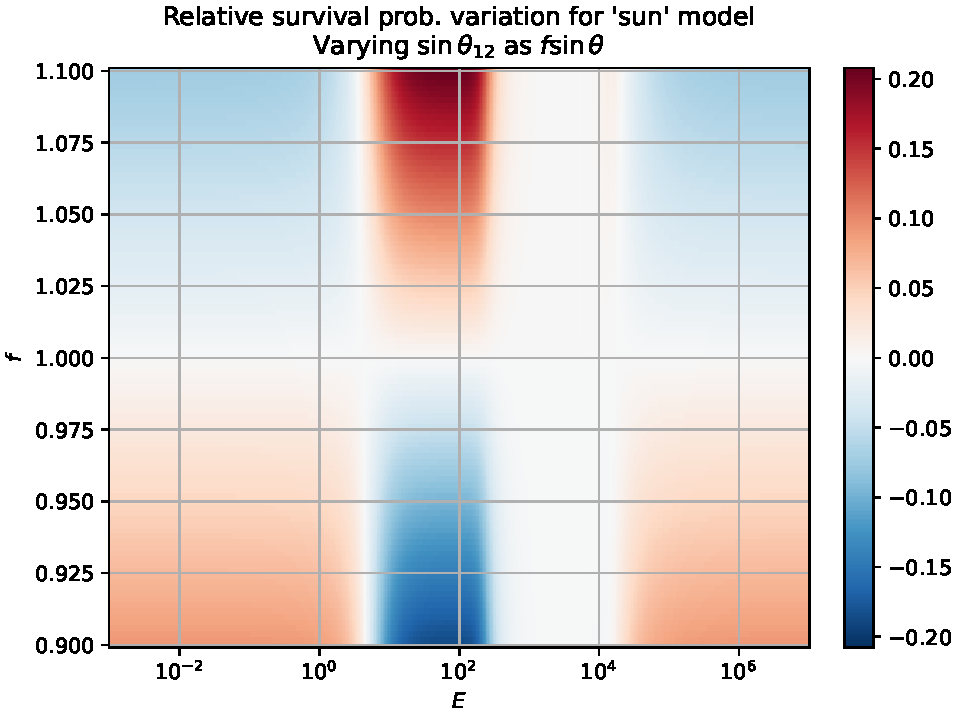
\includegraphics[width=0.8\linewidth]{sun-in-ang12}
		\caption{График относительного отклонения \(\langle P_{ee}\rangle\) при вариации угла \(\theta_{12}\) }
	\end{figure}
\end{frame}

\begin{frame}
	\begin{figure}[h]
		\centering
		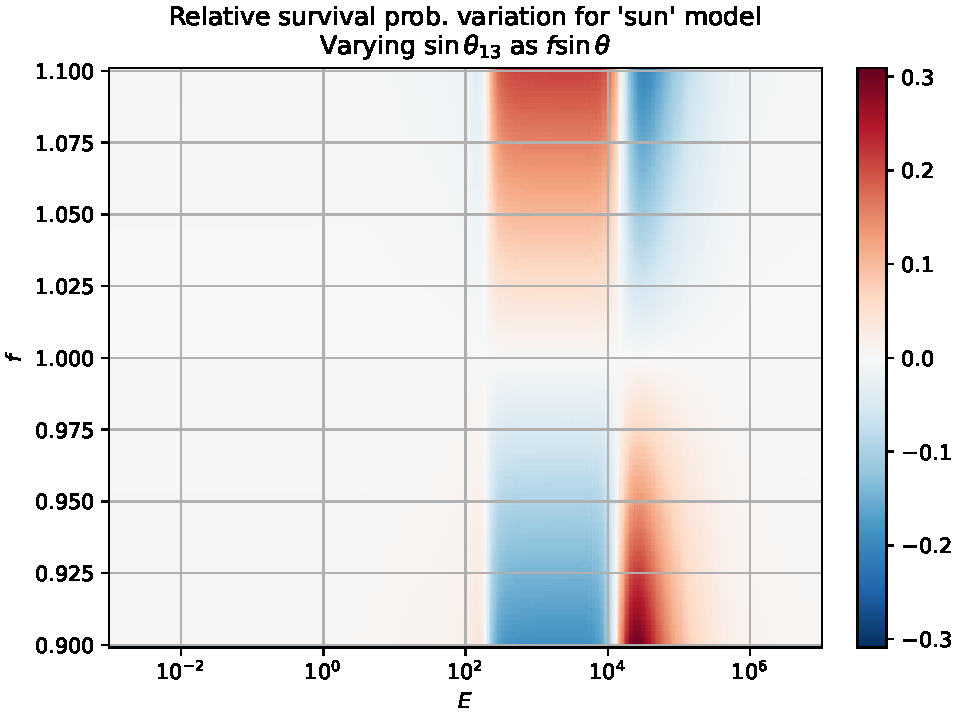
\includegraphics[width=0.8\linewidth]{sun-in-ang13}
		\caption{График относительного отклонения \(\langle P_{ee}\rangle\) при вариации угла \(\theta_{13}\)}
	\end{figure}
\end{frame}

\begin{frame}
	\frametitle{Вывод}
	\begin{itemize}
		\item<1-> Разобран механизм осцилляций нейтрино в вакууме и в веществе.
		\item<2-> Разработаны сценарии для автоматизации расчётов и сценарии для визуализации полученных данных . 
	\end{itemize}
\end{frame}

\begin{frame}
	\frametitle{Перспективы работы}
	\begin{itemize}
		\item<1-> Провести анализ для других типов нейтрино.
		\item<2-> Провести анализ с вариацией параметров профиля плотности.
		\item<3-> Разработать формулы для анализа корреляций в вариациях.
	\end{itemize}
\end{frame}

\begin{frame}
  \frametitle{КОНЕЦ}
  \LARGE\centering\bfseries
  СПАСИБО ЗА ВНИМАНИЕ!
\end{frame}

\begin{frame}
  \frametitle{Дополнительный материал}
\end{frame}

\end{document}

%%% Local Variables:
%%% mode: latex
%%% fill-column: 80
%%% TeX-master: t
%%% TeX-PDF-mode: t
%%% End:
%%% vim: syn=tex ft=tex tw=80 ts=2 sw=2 et:
